\textbf{Цель работы:} измерение зависимости сопротивления полупроводниковых образцов различной формы от индукции магнитного поля. \\

\textbf{Используемое оборудование:} электромагнит, милливеберметр или миллитесламетр (на основе датчика Холла), вольтметр, амперметр, миллиамперметр, реостат, образцы монокристаллического антимонида индия (InSb) $n$-типа.
                    
\section{Теоретическое введение}

В работе исследуется эффект зависимости электрического сопротивления от магнитного поля на примере диска Корбино (см. рис.).

\begin{figure}[h]
    \centering
    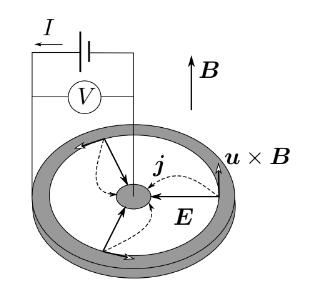
\includegraphics[width = 5 cm]{images/1.png}
    \caption{Диск Корбино}
    \label{karb}
\end{figure}

При отстутствии магнитного поля, направленного перпендикулярно плоскости диска, по диску течёт ток, определяемый по закону 

\begin{equation}
    I = \frac{U}{R_0}, \; R_0 = \frac{\ln{\frac{r_2}{r_1}}}{\sigma_0 2 \pi r h}
\end{equation}

Однако при включении магнитного поля индукции $B$ на частицы-переносчики тока начинает действовать сила Лоренца, из-за чего траектория частиц увеличивается в расстоянии, проходимом между двумя точками с фиксированной разницей потенциалов $U$.

В этом случае проводимость  равна 

\begin{equation}
    \sigma_r = \frac{\sigma_0}{1 + (\mu B)^2}
\end{equation}

Закон Ома преобразовывается в следующий вид:

\begin{equation}
    I = \frac{U}{R}, \; R = R_0 (1 + (\mu B)^2)
\end{equation}

Таким образом, зависимость $I(U)$ поменялась из-за геометрических особенностей диска Корбино. Такой эффект называют геометрическим магнетосопротивлением. В этой работе будут исследоваться зависимость сопротивления диска от магнитного поля, проверяться выше записанные формулы и исследоваться как влияет характер зависимости геометрических форм на зависимость $R(B)$.

\section{Экспериментальная установка}

Для исследование зависимости $R(B)$ используется следующая методика:

\begin{enumerate}
    \item Используется калибровка электромагнита (источника магнитного поля): находится зависимость индукции создаваемого магнитного поля от тока в контуре электродвигателя $B(I_m)$ (или $I_m(B)$), который регистрируется амперметром $A_1$, чтобы в дальнейшем считать величину магнитного поля с помощью тока в контуре $I_m$.
    \item При постоянной силе тока $I_0$, которая настривается с помощью сопротивления реостата в контуре с источником питания, меняется величина индукции магнитного поля, тем самым меняется напряжение $U$, подаваемое на диск Корбино. Исследуется зависимость $R(B)$ через калибровочную кривую и зависимость $U(I_m)$.
    \item Проводится тот же самый опыт с прямоугольной пластинкой с исследованием зависимости её сопротивления $R(B)$.
\end{enumerate}

\begin{figure}[h!]
    \centering
    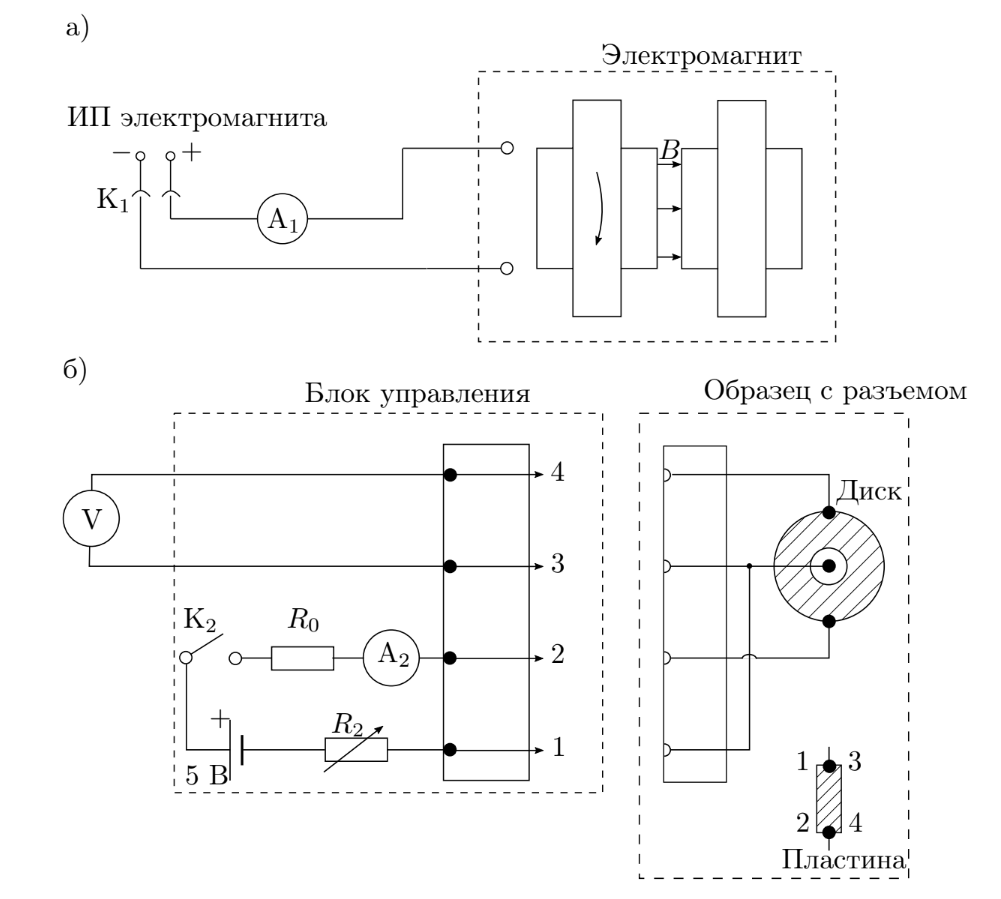
\includegraphics[width = 13 cm]{images/2.png}
    \caption{Схемы экспериментальных установок}
    \label{scheme}
\end{figure}

\section{Ход работы}

\subsection{Построение калибровочной кривой}

Включим милливеберметр и будем снимать зависимость в контуре электродвигателя $I_m(B)$. В нашем случае милливеберметр измеряет не поток магнитного поля, а сразу же напрямую индукцию магнитного поля.

\begin{table}[h!]
    \centering
    \begin{tabular}{|c|c|c|c|c|c|c|}
        \hline
        \textbf{$I$, мА}  & 0         & 10    & 20    & 30    & 40    & 50      \\ \hline
        \textbf{$B$, мТл} & 10,1      & 12,0  & 20,8  & 28,3  & 35,9  & 45,1    \\ \hline

        \textbf{$I$, мА}  & 60        & 70    & 80    & 90    & 100   & -       \\ \hline
        \textbf{$B$, мТл} & 54,4      & 65,0  & 75,7  & 84,9  & 94,6  & -       \\ \hline

        \textbf{$I$, мА}  & 120       & 140   & 160   & 180   & 200   & 220     \\ \hline
        \textbf{$B$, мТл} & 113,9     & 131,3 & 148,7 & 167,0 & 184,9 & 204,0   \\ \hline

        \textbf{$I$, мА}  & 240       & 260   & 280   & 300   & 320   & -       \\ \hline
        \textbf{$B$, мТл} & 220       & 237   & 254   & 269   & 287   & -       \\ \hline

        \textbf{$I$, мА}  & 340       & 360   & 380   & 400   & 420   & 440     \\ \hline
        \textbf{$B$, мТл} & 303,0     & 315,0 & 324,0 & 335,0 & 343,0 & 349,0   \\ \hline


        \textbf{$I$, мА}  & 460       & 480   & 500   & 520   & 540    & -      \\ \hline
        \textbf{$B$, мТл} & 353,0     & 358,0 & 363,0 & 367,0 & 371,0  & -      \\ \hline
    \end{tabular}
    \caption{Таблица данных для калибровочной кривой}
\end{table}

Построим калибровочный график:

\begin{figure}[h!]
    \centering
    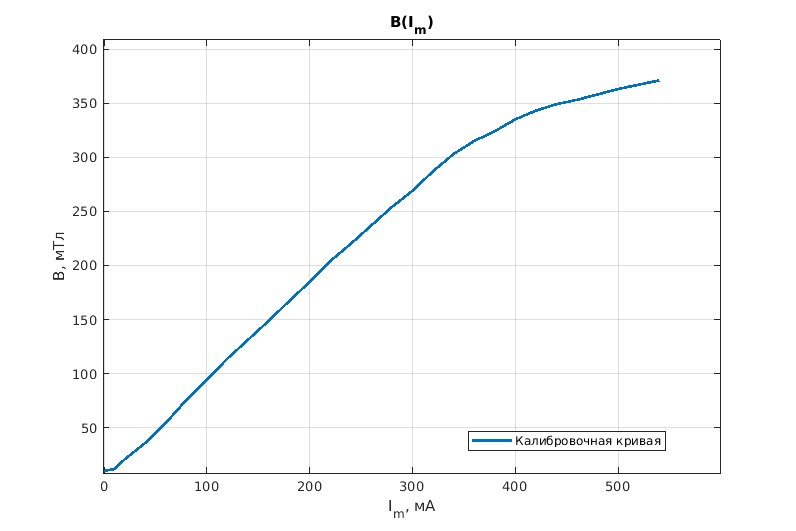
\includegraphics[width = 13 cm]{images/kalibr.png}
    \caption{Калибровочная кривая $B(I_m)$}
    \label{kalib}
\end{figure}

В дальнейшем нужно учесть, что значения индукции магнитного поля сняты с точностью $2 мТл$, а сила тока $5$ мА.

\subsection{Диск Корбино}

Вставим диск Корбино в зазор выключенного электромагнита и измерим падение напряжения $U_0$ в образце при токе $I_0 = 22,5 \pm 0,5$ мА (максимально возможный ток в контуре) через образец: $U_0 = 695 \pm 2$ мВ. Теперь зафиксируем ток в основном контуре (с источником питания) $I_0 = 22,5 \pm 0,5$ мА и будем исследовать $U(I_m)$:

\begin{figure}[h!]
    \centering
    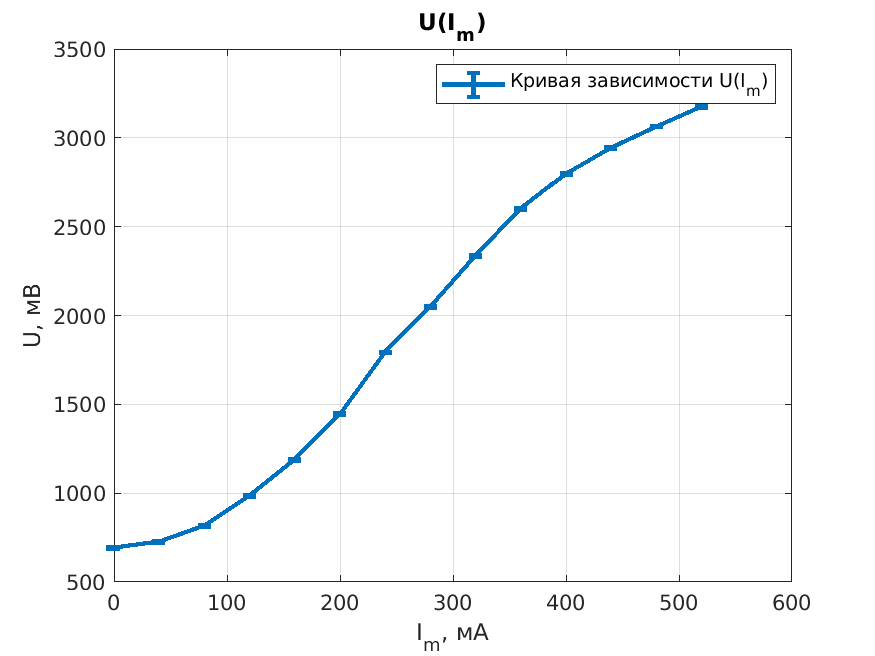
\includegraphics[width = 11 cm]{images/UIM.png}
    \caption{График $U(I_m)$ для диска Корбино}
    \label{uim}
\end{figure}

На графике учтено, что погрешность мультиметра равна $\Delta U = 4$ мВ (учтены данные производителя, ошибка округления и колебания мультиметра около среднего значения), а погрешность амперметра $\Delta I_m = 5$ мА. 

Воспользуемся калибровочной кривой и величиной тока $I_0$, чтобы найти зависимость $R(B)$ (учтена погрешность $\Delta I_0 = 1$ мА).

\begin{figure}[h!]
    \centering
    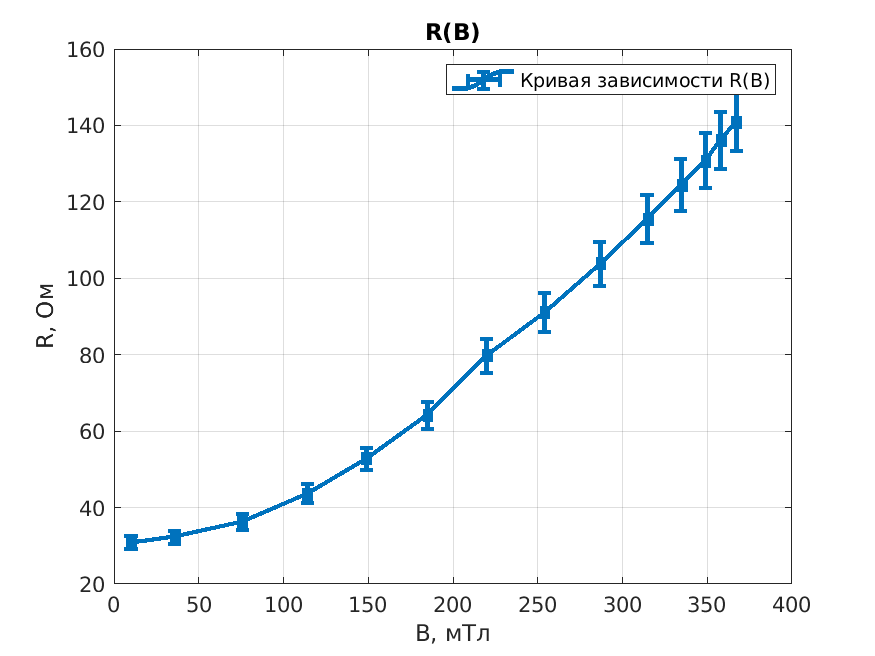
\includegraphics[width = 11 cm]{images/RB.png}
    \caption{График $R(B)$ для диска Корбино}
    \label{RB}
\end{figure}

Теперь построим график $\frac{U - U_0}{U_0}(B^2)$

\begin{figure}[h!]
    \centering
    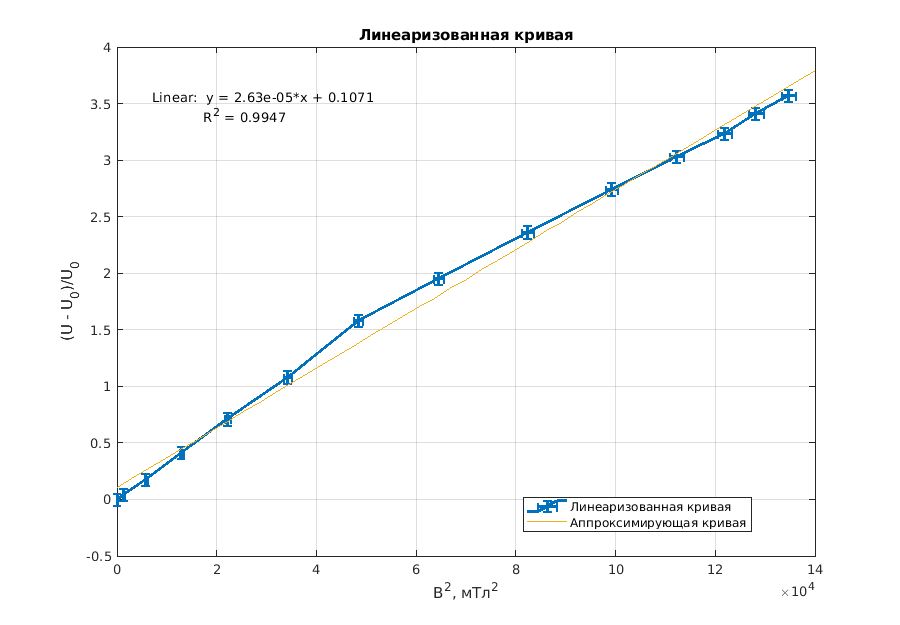
\includegraphics[width = 14 cm]{images/U0B2.png}
    \caption{График $\frac{U - U_0}{U_0}(B^2)$ для диска Корбино}
    \label{U0B2}
\end{figure}

Из графика и коэффициента корреляции видно, что график -- прямая. Значит теоретическая зависимость верна и можно посчитать подвижность зарядов (так как известны погрешности отдельных измерений, но не выполянется $\Delta y \gg \Delta x$, то не получится воспользоваться методом хи-квадрат, используем МНК):

\begin{equation}
    k = \mu^2 = 26,3 \pm 1,8 \; \text{Тл}^{-2} \Rightarrow \mu = 5,13 \pm 0,17 \; \text{Тл}^{-1}
\end{equation}

Заметим, что табличное значение этой величины равно $\mu_{theor} = 7,7 \; \text{Тл}^{-1}$. Возможно, на результат повлияли условия, которые не были устены во время проведения измерений.

При отсутствии магнитного поля сопротивление диска равно $R_0 = 30,9 \pm 1,7$ Ом. Отсюда легко найти удельную проводимость из формулы

\begin{equation}
    R_0 = \frac{\ln{\frac{D}{d}}}{\sigma_0 2 \pi h} \Rightarrow \sigma_0 = \frac{\ln{\frac{D}{d}}}{R_0 2 \pi h} = 513 \pm 18 \; (\text{Ом} \cdot \text{см})^{-1}
\end{equation}

Здест были использованы геометрические размеры диска: $d = 3$ мм, $D = 18$ мм, $h = 1,8$ мм.

Теперь найдём концентрацию носителей тока:

\begin{equation}
    n = \frac{\sigma_0}{e \mu} \thickapprox 6,2 \cdot 10^{18} \; \text{м}^{-3}
\end{equation}

\subsection{Прямоугольная пластина}

Найдём все аналогичные параметры для прямоугольной пластины так же, как и для диска Корбино. Посчитаем сразу линеаризованную зависимость $\frac{U - U_0}{U_0}(B^2)$:

\begin{figure}[h!]
    \centering
    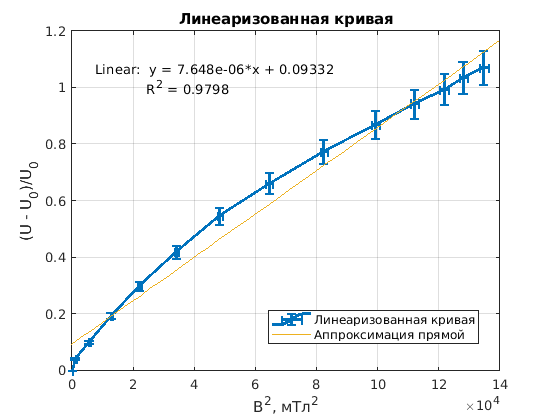
\includegraphics[width = 11 cm]{images/UIMP2.png}
    \caption{График $\frac{U - U_0}{U_0}(B^2)$ для прямоугольной пластины (параллельное расположение)}
    \label{uimp1}
\end{figure}

Из коэффициента корреляции понятно, что зависимость нельзя считать линейной. Значит изначальная теоретическая зависимость тоже не выполняется. Выходит, что она специфична для геометрической формы диска Корбино. Построим аналогичный график для перпендикулярного расположения пластины:

\begin{figure}[h!]
    \centering
    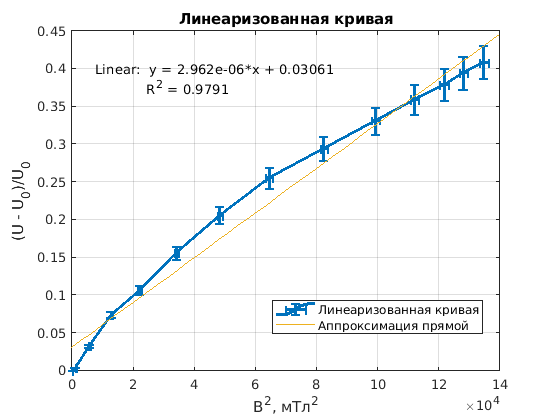
\includegraphics[width = 11 cm]{images/UIMP1.png}
    \caption{График $\frac{U - U_0}{U_0}(B^2)$ для прямоугольной пластины (перпендикулярное расположение)}
    \label{uimp2}
\end{figure}

Понятно, что этот случай и должен был отличаться только коэффициентами зависимости. 

\section{Заключение}

Теоретическая зависимость $R(B)$ действительно выполняется для диска Корбино. Полученный коэффициент зависимости, который равен подвижности носителей зарядов, отличается от табличного даже с учётом погрешности ($\mu = 5,13 \pm 0,17 \; \text{Тл}^{-1}$, $\mu_{theor} = 7,7 \; \text{Тл}^{-1}$). Отсюда можно сделать вывод, что либо не были учтены какие-то внешние факторы при снятии данных, либо исследуемый материал не является монокристаллическим антимонидом индия (InSb).

Квадратичная зависимость $R(B)$ действительно специфична для диска Корбино из-за его геометрических форм, так как для прямоугольной пластинки эта зависимость неверна (в любом её расположении).






